%=======================+=========================
%================   Solenoid  ================
%=================================================

\section[Solenoid Magnet]{Solenoid magnet 
  \label{sec:solenoid}
}

\subsection[Overview]{Overview \label{sec:sol:overview}
}

The core of the GlueX spectrometer is a superconducting magnetic
solenoid with a bore of about 2~m in diameter and the overall
yoke's length of about 4.8~m. The photon beam passes along the axis of
the solenoid.  At the nominal current of 1350~A used for the GlueX
experiment the magnet provides a $\approx$2~T field at its axis.

The magnet was designed and built at SLAC in the early
1970's~\cite{Alcorn-confer-1972} for the LASS
spectrometer~\cite{Aston:1987uc}. It is a cryostatically
stable design and uses cryostats that were designed to be opened and
serviced with hand tools. It was refurbished and modified%
\footnote{
  The front plate of the flux return yoke was modified, leading to a
  swap of the two front coils and modifications of the return flux
  yoke in order to keep the magnetic forces on the front coil under
  the design limit.  The original gaps between the yoke's rings were
  filled with iron. The Cryogenic Distribution Box was designed and
  built anew.
} 
for the GlueX experiment~\cite{Ballard:2011tm, Ballard:2015wma}. 

The magnet is constructed of four separate superconducting coils and
cryostats. The flux return yoke is made of several iron rings.  The
coils are connected in series. A common liquid helium tank is located
atop the magnet providing the gravity feed of the liquid to the
coils. The layout of the coils' cryostats and the flux return iron
yoke is shown in Fig.~\ref{fig:layout_spectrometer}.
Table~\ref{tab:sol:summary} summarizes the important magnet
parameters.

% ======================================================================================
  

\begin{table}[h]
 \begin{center}
   \small
   \begin{tabular}{lr}
     \hline
     \hline
       Inside diameter of coils        & 2032 mm \\
       Clear bore diameter             & 1854 mm \\
       Overall length along iron       & 4795~mm \\
       Inside iron diameter            & 2946~mm \\
       Outside iron diameter           & 3759~mm \\
       Original yoke, cast and annealed - steel & AISI 1010 \\
       Added filler plates - steel     & ASTM A36 \\
       Full weight                     & 284~t      \\
       Full number of turns            & 4608 \\
       Number of separate coils        & 4 \\
%       Longitudinal arrangement of coils & 1-2-3-4 & & 2-1-3-4 \\
       Turns per coil 2                &  928 \\   
       Turns per coil 1                & 1428 \\   
       Turns per coil 3                &  776 \\   
       Turns per coil 4                & 1476 \\   
       Total conductor weight          & 13.15 t \\
       Coil resistance at $\sim$300~K & 15.3~$\Omega$ \\   
       Coil resistance at  $\sim$10~K & $\sim$0.15$\Omega$ \\   
       Design operational current      & 1500 A \\
       Nominal current (actual)        & 1350 A \\
       Maximal central field at 1350~A & 2.08 T \\   
       Inductance at 1350~A            & 26.4 H \\
       Stored energy at 1350~A         & 24.1 MJ  \\
       Protection circuit resistor     & 0.061 $\Omega$  \\
%       Total conductor length        & 117600 ft & 35.84 km & {\it same} \\
%       Substrate material            & \multicolumn{1}{r}{Copper} & & {\it same} \\   
%       Copper-to-filament ratio (A)  & \multicolumn{1}{r}{20:1} & & {\it same} \\   
%       Copper-to-filament ratio (B)  & \multicolumn{1}{r}{28:1} & & {\it same} \\   
       Coil cooling scheme             & helium bath \\   
       Total liquid helium volume      & 3200 $\ell$ \\
       Operating temperature (actual)  &  4.5~K \\   
       Refrigerator liquefaction rate at 0~A        & 1.7~g/s    \\
       Refrigerator liquefaction rate at 1350~A     & 2.7~g/s    \\
%       Refrigerator liquefaction rate at 0~A        & 1.7~g\thinspace{}s$^{-1}$    \\
%       Refrigerator liquefaction rate at 1350~A     & 2.7~g\thinspace{}s$^{-1}$    \\
%       Protection circuit limiting voltage & 500 V & & 90 V \\
     \hline
   \end{tabular}
   \normalsize
 \end{center}
  \caption{
    The actual parameters of the solenoid.  The units are metric. The
    coils are ordered along the beam direction.
    \label{tab:sol:summary}
  }
\end{table}


\subsection[Conductor and Coils]{Conductor and Coils
 \label{sec:sol:coils}
}

The superconductor composite is made of niobium--titanium filaments
%\footnote{The critical temperature is about 10$^\circ$K.} 
in a copper substrate, twisted and shaped into a
$\sim$7.62$\times$1~mm$^2$ rectangular band. The laminated conductor
is made by soldering the superconductor composite band between two
copper strips
%\footnote{Copper CDA 102. Average Resistivity Ratio for
%  300$^\circ$K:4.2$^\circ$K is a minimum of 150:1, claimed by the builders of the
%  magnet\cite{Solen-conductor}. 
%  %It contradicts the data from another
%  %source\cite{CuHandbook}, which specifies $10<$RRR$<100$ for ETP
%  %copper. 
%  Our measurements show RRR$\approx{}$100.
%} 
to form a rectangular cross section of 7.62$\times$5.33~mm$^2$
%\cite{Alcorn-confer-1972}.  
The measured resistivity ratio of the conductor at $\sim{}300^\circ{}$K and
$\sim{}15^\circ{}$K is $\approx{}$100.  
%Two types of filaments have
%been used (see Fig.~\ref{fig:sol:conductor-cartoon} and
%Table.~\ref{tab:sol:conductor}). The Grade A conductor provides a higher
%current limit than the Grade B conductor and is used in the area of
%the highest magnetic field (Coil 4).

%The coil was wound on G-10 standoff strips glued on the cylindrical
%inner wall of the liquid helium vessel.  
As the coil was wound, a 0.64~mm-thick stainless steel support band
and two 0.2~mm-thick Mylar insulating strips were wound along with it
for pre-tensioning and insulation%
%(Fig.~\ref{fig:sol:conductor-cartoon})
. 
The liquid helium is in contact with the shorter (5.33~mm) sides of
the cable.

Each of the coils consists of a number of subcoils. Each subcoil
contains a number of ``double pancakes'' with the same number of
turns.
%(see Table~\ref{tab:sol:coils-turns}). 
Each double pancake is made from a single piece of conductor. The
voltage across the subcoils is monitored using special wires passing
through the coils' chimneys along with the helium supply pipes and the
main conductor.

The cold helium vessel containing the coil is supported within its
warm cryostat vacuum vessel by a set of columns designed to provide
sufficient thermal insulation. The columns are equipped with strain
gauges for monitoring the stresses on the columns. The helium vessel
is surrounded by a nitrogen-cooled shield made of copper panels.
Super-insulation is placed between the vacuum vessel and the nitrogen
shield.  The vacuum vessels are attached to the matching iron rings of
the yoke.

The power supply%
\footnote{Danfysik System 8000 Type 854.}
provides up to 10~V DC for ramping up/down the current. It also
includes a protection circuit, which can be fired by the quench
detector as well as by other signals.  A relatively low dump resistor
of 0.061~$\Omega$ limits the maximal voltage on the magnet during
trips to 100~V. The dumping time constant of $L/R \approx 7$~min is
relatively long, but safe according to the original design of the
magnet. A large copper mass and the helium bath are able to absorb a
large amount of energy during a quench without overheating the solder
joints. This allowed for a relatively slow-reacting - 0.5~s decision
time - but more noise-proof and ``intelligent'' quench detector.  The
quench detector compares the measured voltages on different subcoils
in order to detect a resistive component that might appear in a
subcoil.
%The decision is made based on the measured voltages on the
%subcoils.  
During ramping the current up or down such a voltage is proportional
to the subcoil's inductance.  Relative values of inductance of various
subcoils depend on the value of the current because of saturation
effects in the iron yoke. There are also transient effects at changes
of the slew rate caused by Foucault currents in the yoke.
%The quench detector compares
%voltages on different subcoils in order to detect a resistive
%component that might appear in a subcoil.  
The system includes two redundant detectors - one uses analog signals
and a simplified logic, another is done in the PLC control system (see
Section~\ref{sec:sol:controls}) which uses digitized signals. The PLC
digital programmable device is more sensitive since it takes into
account the dependence of the coils' inductance on the current and
provides a better filtering of the noise.  The ramping slew rate is
limited by the transient imbalance of the voltages on subcoils, that
may trigger the quench detector. Additionally, $\sim$1~ms-long voltage
spikes of unidentified origin have been observed in coil 2 at high
slew rates, also triggering the quench detector. Powering up the
magnet to 1350~A takes about 8~h.

For diagnostic purposes two 40-turns pickup coils are installed on the bore
surface of the vacuum vessel of each of the coils. 

\subsection[Cooling System]{
   Cooling System
   \label{sec:sol:cryo}
}

The cooling system is described in detail in Ref.~\cite{Lavendure:2014:refrig}.
A standalone helium refrigerator located
in a building adjacent to Hall D provides liquid helium and nitrogen
via a transfer line to the Cryogenic Distribution Box atop the
magnet. The transfer line delivers helium at 2.6~atm and 5~K to a Joule-Thomson
(JT) valve providing liquid to a cylindrical common helium tank in the
Distribution Box. The level of liquid helium in the tank is measured
with a superconducting wire probe%
\footnote{
  American Magnetics Model 1700 with HS-1/4-RGD-19"/46"-4LDCP-LL6-S sensor
}
 and is kept at about half of the tank's diameter. The cold helium gas
 from the tank is returned to the refrigerator which keeps the
 pressure at the top of the tank at 1.2~atm corresponding to about
 4.35~K at the surface of the liquid%
\footnote{
  The original implementation at SLAC did not recycle the helium and
  operated at atmospheric pressure.
}
.
Each coil is connected to the common helium tank by two vertical 2-inch
pipes.  One pipe is open at the bottom of the tank while the other one
is taller than the typical level of helium inside the tank. The main
conductor and the wires for voltage monitoring pass through the former
pipe. Additionally, two $\sim$6~m long, 3/8~inch ID pipes go outside
the coil's helium vessel, from the Distribution Box to the bottom of
the coil. One of those pipes is connected to a JT valve in the Box,
and is used to fill the coil initially and is not used during operations.
Another one reaches the bottom of
the common helium tank in order to provide 
a thermosyphon effect essential
for the proper circulation of helium in the coil. The main current is
delivered into the helium tank via vapor-cooled leads and is
distributed to the coils by a superconducting cable. After cooling the
leads the helium gas is warmed up and returned to the refrigeration
system. The gas flow through the leads is regulated depending on the
current in the magnet and at 1350~A the flow is about 0.25~g/s. The
coils and the Distribution Box are equipped with various sensors for
temperature, pressure, voltage, and flow rates.

\subsection[Measurements and Controls]{
         Measurements and Controls
        \label{sec:sol:controls}
}

The control system for the superconducting solenoid, the power supply, 
and the cryogenic system, is based on Programmable Logic
Controllers (PLC)%
\footnote{
  Allen-Bradley Programmable Logic Controllers
  \url{http://ab.rockwellautomation.com/Programmable-Controllers}.
}%
.
The PLC digitizes the signals from various sensors, communicates with
other devices, reads out the data into a programmable unit for
analysis, and sends commands to various devices. Additionally, it is
connected to EPICS in order to display and archive the data (see
Section \ref{sec:controls}).  The practical sampling rate of a
sensor's readout is limited to a few Hz, which is too low for
detection of fast voltage spikes on the coils due to motion, shorts,
or other effects. Therefore, the voltage taps from the coils
and the pickup coils are read
out by a PXI%
\footnote{
  National Instruments, PXI Platform, \url{http://www.ni.com/pxi/}.
}%
system, which provides an initial sampling rate of about 100~kHz. The
PXI system also reads out several accelerometers attached to the
coils' chimneys, which may detect a motion inside the coils. The PXI
CPU performs initial integration and arranges the data in time-wise
rows with a sampling rate of 10~kHz.  The PLC system reads out these
data from the PXI system. Additionally, the PXI data are read out by
an EPICS server at the full 10~kHz sampling rate and are recorded 
to files for further analysis.

\subsection[Field Calculation and Measurement]{
         Field Calculation and Measurement
        \label{sec:sol:field}
}

The momentum resolution of the GlueX spectrometer is larger than
1\% and is dominated by multiple scattering and the spatial
resolution of the coordinate detectors.  A fraction of a percent is a
sufficient accuracy for the field determination.  The coils are
axially symmetric while the flux return yoke is nearly axially
symmetric, apart from the holes for the coil's chimneys. The field was
calculated using a 2-dimensional field calculator {\it
  Poisson/Superfish}%
\footnote{
   Poisson/Superfish developed at LANL,
   \url{https://laacg.lanl.gov/laacg/services/serv_codes.phtml\#ps}.
} 
, assuming axial symmetry.  The model of the magnet included the
fine structure of the subcoils and the geometry of the yoke
iron. Different assumptions about the magnetic properties of the yoke
iron have been used: the {\it Poisson} default AISI 1010 steel, the
measurements of the original yoke iron made at SLAC, and the 1018
steel for the filler plates. Since the results of the field
calculations differ for less than 0.1\% the default {\it Poisson} AISI
1010 steel properties for the whole yoke iron were used for the final
field map calculations.

The 3 projections of the magnetic field have been measured along lines
parallel to the axis, at 4 values of the radius and at up to 6 values
of the azimuthal angle. The calculated field and its deviation from
the measurements are shown in Fig.~\ref{fig:sol:field_comparison}. The
tracking detectors occupy a volume of $R<56$~cm and $45<Z<340$~cm. In
this volume the field deviation at $R=0$ does not exceed 0.2\%. The
largest deviation of 1.5\% is observed at the downstream edge of the
fiducial volume and at the largest radius. Such a field uncertainty in
that region does not affect noticeably the momentum resolution. In
most of the fiducial volume the measured field is axially symmetric to
$\approx$0.1\% and deviates from this symmetry by $\approx$2\% at the
downstream edge and the largest radius.

The calculated field map is being used for the track reconstruction and
physics analysis.
   
% ======================================================================================

%\begin{figure}[tp]
\begin{figure}[!htb]
  \begin{center}
     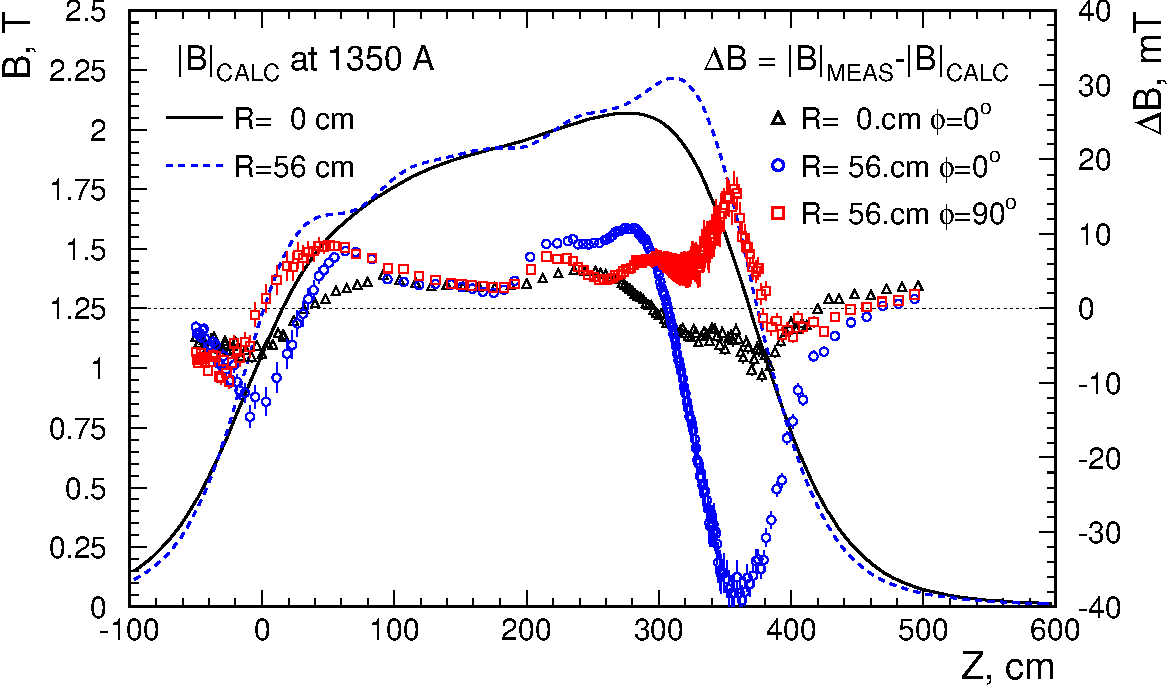
\includegraphics[angle=0,width=1.0\linewidth]{figures/solenoid_field_calc-meas_comparison_7_1_01}%
  \end{center}
  \caption{
    The full field at 1350~A calculated with {\it Poisson} (the left
    scale) at the axis and at the edge of the tracking fiducial volume
    - R=56~cm. The deviations of the measurements from the
    calculations are shown (the right scale) at the axis, as well as
    at R=56~cm. The measurements have been done at 6 azimuthal
    angles. Those demonstrating the largest deviations from the
    calculations - at 0$^\circ$ and 90$^\circ$ - are shown.  
%    In the area most important for tracking $45<Z<320$~cm the
%    deviations from the calculations are below 0.5\%.
    \label{fig:sol:field_comparison}
  }
\end{figure}


% ----------------------------------------------------------------------
